% ------------------------------------------------------------------------
% file `math2-exercise-9-exercise-body.tex'
%   in folder `xsim/'
%
%     exercise of type `exercise' with id `9'
%
% generated by the `exercise' environment of the
%   `xsim' package v0.11 (2018/02/12)
% from source `math2' on 2021/10/28 on line 217
% ------------------------------------------------------------------------
L'ensemble des élèves de deuxième année et 5 professeurs aimeraient partir en excursion dans un parc d'attracions.
    \begin{tasks}
        \task Sachant qu'il y a 225 élèves en deuxième année, et qu'un car ne peut transporter que 35 personnes, combien de cars faudra-t-il réserver? Ecris tous tes calculs.\\
        %Laisser de l'espace
        \task Combien de places resteront inoccupées?\\
        %Laisser de l'espace
        \task Voici un tableau reprenant les tarifs dans le parc d'attraction. Combien faudra-t-il débourser à la caisse? Ecris tous tes calculs.\\
        \centering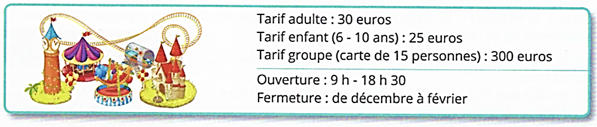
\includegraphics{diviseurs-et-multiples/imgd/prix.png}
        %laisser de l'espace
    \end{tasks}
